\section{Teori}\label{sec:theory} 
Den teori som presenteras i detta kapitel är den teori som är relevant för att förstå de tekniker och verktyg som används i arbetet.


\subsection{Kunskapsgraf}\label{subsec:Kunskapsgraf}

En kunskapsgraf är en strukturerad representation av information i form av ett nätverk av verkliga entiteter.
Dessa entiteter kan vara objekt, händelser och begrepp och tillsammans illustrerar nätverket relationerna mellan dem.
Informationen lagras vanligtvis i en grafdatabas och visualiseras som en grafstruktur~\cite{21}.

En kunskapsgraf består av tre huvudkomponenter: noder, kanter och etiketter.
Noden representerar en enskild entitet,
kanten representerar relationen mellan två noder, och etiketten beskriver vad noderna och relationerna representerar, exempelvis \textit{Person} eller \textit{Arbetar på}~\cite{21}.

Kunskapsgrafer är särskilt användbara i situationer där data är starkt sammankopplad och där relationerna i sig bär viktig information.
 De används exempelvis inom rekommendationssystem, bedrägeridetektion och i detta fall för att underlätta informationssökning.
Genom att integrera data från olika källor och organisera den utifrån tydliga samband kan kunskapsgrafer bidra till att synliggöra mönster och insikter som annars kan vara svåra att upptäcka~\cite{5}.

\subsubsection{Grafdatabasen Neo4j}

Grafdatabaser är en typ av databashanteringssystem som representerar data i form av noder och relationer.
Till skillnad från traditionella relationsdatabaser är relationerna en central del av datamodellen, vilket bidrar till effektiv traversering av data (s.~6)~\cite{robinson2015graph}.

Grafdatabaser baseras på riktade grafer, vilket innebär att varje relation har en startnod och därmed en definierad riktning.
Denna riktning används för att beskriva semantiken i relationen mellan två noder.
Trots detta kan relationer traverseras i båda riktningarna vid frågeställning~\cite{10}.

Det är inte heller nödvändigt att alla noder i en graf är direkt kopplade till varandra, utan en graf kan bestå av flera sammanhängande delgrafer.

I Figur \ref{fig:visualisation} visas ett utdrag från den skapade grafdatabasen där två personer är kopplade till ett projekt medan en person är kopplad till ett annat.
\begin{figure}[H]
    \centering
    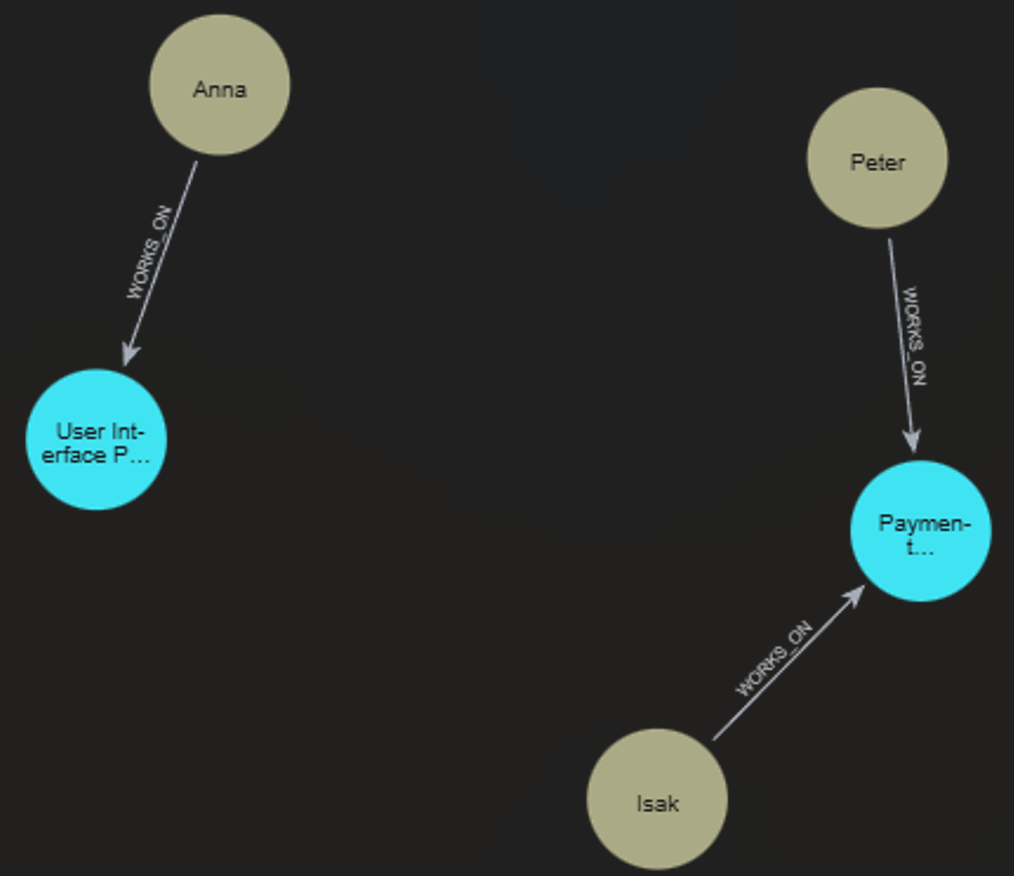
\includegraphics[width=0.8\textwidth]{Figures/corre.png}
    \caption{Visualisering av en del av den skapade grafdatabasen}
    \label{fig:visualisation}
\end{figure}

Neo4j är grafdatabasen som används i detta projekt för att implementera kunskapsgrafen. I Neo4j är grafstrukturen implementerad direkt i databasen på lagringsnivå, och inte ovanpå en annan databasmodell.
Detta innebär att data lagras direkt i grafstrukturen och inte i en separat struktur~\cite{6}.

\subsubsection{Cypher}
Cypher är det frågespråk som används i Neo4j. Det är ett deklarativt frågespråk för grafdatabaser ursprungligen utvecklat för just Neo4j.
Språket är utformat för att uttrycka frågor genom mönstermatchning, vilket gör det möjligt att formulera graftraverseringar på ett naturligt sätt~\cite{11}.

Till skillnad från SQL, som använder join-operationer för att koppla samman
  tabeller, uttrycker Cypher graftraverseringar direkt i frågesyntaxen vilket bidrar till mer intuitiva och läsbara frågor. Språket
  stödjer även skapande, uppdateringar och borttagning av data i grafen~\cite{11}.

Nedan visas ett exempel på en Cypher-fråga som hämtar alla Repository-noder
  som är kopplade till en Person via relationen WORKS\_ON:

\begin{verbatim}
MATCH (p:Person)-[:WORKS_ON]->(r:Repository)
RETURN r
\end{verbatim}

Syntaxen speglar grafstrukturen direkt. Parenteser representerar noder och pilar representerar relationer, vilket gör frågorna lätta att läsa och förstå.

\subsection{Large Language Model (LLM)}\label{subsec:LLM}
En LLM är en typ av artificiell intelligensmodell som är tränad på stora mängder data.
 Detta gör dem kapabla till att förstå det mänskliga språket samt andra typer av innehåll för att kunna utföra olika typer av arbetsuppgifter~\cite{12}.

I detta projekt används LLM:en för att tolka en användares fråga och sedan avgöra vilket eller vilka verktyg som ska användas för att hämta rätt information från antingen grafdatabasen eller systemens API:er.
Den används även för att generera de Cypher-frågor som körs mot grafdatabasen.

\subsection{Model Context Protocol (MCP)}\label{subsec:mcp_theory}
Model Context Protocol (MCP) är ett protokoll som används för att koppla samman LLM:er med externa system.
Genom att använda sig av MCP kan LLM:erna få tillgång till den skapade grafdatabasen och andra externa datakällor~\cite{13}.
Detta gör det enklare att utveckla AI-applikationer utan att behöva skapa specialiserade gränssnitt för varje datakälla eller modell~\cite{4}.

Istället för att modellen har direkt tillgång till alla datakällor, fungerar MCP som ett mellanlager där funktionalitet exponeras i form av verktyg.
Dessa verktyg kan sedan användas för att hämta data från databaser, anropa API:er eller utföra andra typer av operationer.

När en användare ställer en fråga kan LLM:en tolka frågan och avgöra vilket eller vilka verktyg som behöver användas för att samla in relevant information.
Resultatet från dessa anrop används sedan som underlag för att generera ett svar till användaren.

MCP möjliggör därmed utvecklingen av AI-applikationer där LLM:er fungerar som agenter som aktivt hittar och hämtar information från källor~\cite{4}.

\subsubsection{Programvarubibliotek (SDK)}
För att implementera MCP-servern används ett programvarubibliotek (SDK) som erbjuder nödvändig funktionalitet.
Ett SDK är en komplett uppsättning verktyg som gör det möjligt för utvecklare att bygga programvara för en specifik plattform.
Det innehåller bland annat byggstenar, ramverk, kodexempel, felsökningsverktyg och dokumentation~\cite{14}.

I projektet används MCP SDK~\cite{15} för att skapa servern, sessioner och verktyg som LLM:en kan använda.

\subsubsection{Kommunikation över Hypertext Transfer Protocol (HTTP)}
Kommunikationen mellan LLM:en och MCP-servern sker genom Cherry Studio över Hypertext Transfer Protocol (HTTP) genom ett request/response-baserat gränssnitt.
När LLM:en anropar ett verktyg skickar Cherry Studio en förfrågan till MCP-servern som utför den begärda operationen och returnerar resultatet~\cite{16}.

Denna modell bidrar till en tydlig separation mellan LLM:en och datakällorna, där MCP-servern fungerar som en mellanhand som hanterar de externa anropen.
Genom att använda HTTP-gränssnittet blir systemet flexibelt och kan integreras med flera olika klienter och tjänster.

\subsection{API-baserad dataåtkomst}\label{subsec:api}
I lösningen som används för att jämföra mot grafbaserade lösningen används en API-baserad dataåtkomst där verktygen i MCP-servern tillhandahåller kod för att göra olika API-anrop för att hämta data från olika datakällor.
Detta innebär att istället för att ha en centraliserad databas där all data är lagrad, så hämtas data i realtid från olika källor när det behövs.

\subsection{Externa datakällor}\label{subsec:external_sources}
De tre externa systemen GitHub, Slack och Confluence utgör de informationskällor som arbetet utgår ifrån.
Den API-baserade lösningen hämtar data direkt från dessa systems API:er, medan den grafbaserade lösningen innehåller syntetisk
  data modellerad efter den typ av information som finns i respektive system.

\subsubsection{GitHub}\label{subsubsec:github}
GitHub är en plattform för att lagra och hantera kodprojekt.
Den används av utvecklare för att samarbeta, dela kod och hantera versioner av sina projekt.
Plattformen tillhandahåller verktyg för versionshantering, kodgranskning, ärendehantering och projektledning, vilket gör den lämplig för både öppen källkod och professionella arbetsflöden~\cite{github}.

I detta arbete används GitHub som en av de externa datakällorna.
Det bidrar med information om projekt (repositories), tillagd/ändrad kod (commits), problem (issues) och aktiva användare.

\subsubsection{Slack}\label{subsubsec:slack}
Slack är en kommunikationsplattform för organisationer som samlar meddelanden, filer, användare och data på ett ställe.
Den används för att underlätta samarbete och kommunikation inom team och organisationer, och erbjuder funktioner som kanaler, direktmeddelanden, filöverföring och integrationer med andra verktyg~\cite{slack}.

I detta arbete används Slack som en av de externa datakällorna för att bidra med information om användare, kanaler och meddelanden.

\subsubsection{Confluence}\label{subsubsec:confluence}
Confluence är en plattform som centraliserar teamets kunskap och samarbete i en gemensam arbetsyta.
Den används för att skapa, organisera och dela dokumentation, planer och annan information inom en organisation~\cite{confluence}.

I detta arbete används Confluence för att bidra med information om teams, dokumentationssidor och författare.

\subsection{Cherry Studio}\label{subsec:CherryStudio}
Cherry Studio är en plattform som används för att interagera med LLM:er genom ett grafiskt användargränssnitt. Plattformen stödjer flera 
olika modeller och möjliggör konfiguration av externa integrationer exempelvis MCP~\cite{7}.

I detta arbete används Cherry Studio som klient för att skicka och få svar av LLM:en, samt för att koppla samman LLM:en med den skapade MCP-servern.
Genom denna integration får LLM:en tillgång till de verktyg som i sin tur har tillgång till grafdatabasen och API:erna.

Cherry Studio fungerar därmed som gränssnittet mellan användaren och systemets backend, där LLM:en blir en central komponent för att tolka och besvara användarens frågor.

\subsection{Relaterat arbete}

I detta underkapitel presenteras tidigare forskning och arbete som är relevant för detta projekt.

\subsubsection{Kunskapsgrafer som kontextkällor för LLM:er i utbildningssystem}

Arbetet undersöker hur kunskapsgrafer kan användas som faktakällor för att minska hallucinationer i LLM-genererade svar inom utbildningssystem.
Författarna visar att en LLM som har tillgång till strukturerad kontext från en kunskapsgraf levererar mer korrekta och relevanta förklaringar jämfört med när modellen enbart förlitar sig på träningsdata~\cite{relWork}.

Studien bygger, liksom detta arbete, på att ge en LLM strukturerad kontext från en kunskapsgraf för att förbättra dess förmåga att hämta och använda information.
Skillnaden är att studien fokuserar på att minska hallucinationer inom utbildningen, medan detta arbete fokuserar på informationshämtning inom en organisation.

\subsubsection{GraphRAG för frågefokuserad sammanfattning}

Arbetet undersöker hur en grafbaserad RAG-lösning (Retrieval-Augmented Generation) kan förbättra LLM:ers förmåga att besvara globala frågor riktade mot en samling textdokument.
Metoden går ut på att låta en LLM automatiskt bygga kunskapsgrafen med entiteter och relationer från dokumenten,
 och sedan dela in dessa i olika kluster där varje kluster sedan sammanfattas av LLM:en.
När en fråga ställs används dessa sammanfattningar som kontext till LLM:en för att generera ett svar.
Resultaten visar att detta tillvägagångssätt presterar bättre än vanlig RAG på globala frågor som kräver förståelse för hela datasetet~\cite{edge2024graphrag}.

Liksom detta arbete bygger GraphRAG på principen att en kunskapsgraf ger LLM:en bättre förutsättningar att navigera och kombinera information jämfört med att söka i ostrukturerad data.
Skillnaden är att GraphRAG bygger grafen automatiskt från ostrukturerad text och fokuserar på dokumentsammanfattning, medan detta arbete utgår från en manuellt modellerad kunskapsgraf med syfte att koppla samman organisatorisk information från olika datakällor.


